\documentclass[12pt]{article}
\usepackage{graphicx}
%\documentclass[journal,12pt,twocolumn]{IEEEtran}
\usepackage[none]{hyphenat}
\usepackage{graphicx}
\usepackage{listings}
\usepackage[english]{babel}
\usepackage{graphicx}
\usepackage{caption}
\usepackage{hyperref}
\usepackage{booktabs}
\usepackage{array}
\usepackage{amsmath}   % for having text in math mode
\usepackage{listings}
\lstset{
  frame=single,
  breaklines=true
}
%New macro definitions
\newcommand{\mydet}[1]{\ensuremath{\begin{vmatrix}#1\end{vmatrix}}}
\providecommand{\brak}[1]{\ensuremath{\left(#1\right)}}
\providecommand{\norm}[1]{\left\lVert#1\right\rVert}
\newcommand{\solution}{\noindent \textbf{Solution: }}
\newcommand{\myvec}[1]{\ensuremath{\begin{pmatrix}#1\end{pmatrix}}}
\let\vec\mathbf

\begin{document}
\begin{center}
\textbf\large{CLASS-10\\CHAPTER-7 \\ COORDINATE GEOMETRY}
\end{center}

\section*{EXERCISE - 7.4}

\begin{enumerate}
\item lf $(-4,3)\text{ and }(4,3)$ are two vertices of an equilateral triangle,find the coordinates of the third vertex,given that tne origin lies in the interior of the triangle 
\item $\vec{A} (6,1),\vec{B}(8,2) \text{ and } \vec{C}(9,4)$ are three vertices of a parallelogram $\vec{ABCD}$ .lf $\vec{C}$ is the midpaint of $\vec{DC}$ find the area of $\triangle \vec{ADE}$
\item the points $\vec{A} (x_1,y_1),\vec{B}(x_2,y_2)\text{ and } \vec{C} (x_3,y_3) $ are the vertices of $\triangle\vec{ABC}$
	\begin{enumerate}	
		\item The median from $\vec{A}$ meets $\vec{BC}$ at $\vec{D}$ find the coordinates of the point $\vec{D}$
		\item Find the coordinates of the point p  on $\vec{AD}$ such tnat $\vec{AP}.\vec{PD}$=2
\item Find the coordinates of points $\vec{Q}$ and $\vec{R}$ an medians $\vec{BE}\text{ and }\vec{CF}$respectively such that $\vec{BQ}:\vec{QE}=2;1$ and $\vec{CR}\vec{RF}=2;1$
\item What are the coordinates of the centroid of the triangle $\vec{ABC}$
	\end{enumerate}
\item If the points  $\vec{A} (1,-2) \vec{B}(2,3) \vec{C}(a,2)\text{ and }\vec{D} (-4-3)$ form pamrallelogram,find the vale of a and height of the parallelogram taking $\vec{AB}$ as base.
\item Students of a school are standing in rows and colums in their playgreound for a drill practice $\vec{A,B,C}$ and Dare the positions of four students as showh in figure 7,4. is it passible to place jaspal in the drill in such a woy tnat he is equidisthant from each of the four students $\vec{ A,B,C}$ and $\vec{D}$ lf so ,what should be his position 
\item Ayush starts walking from his house to office. lnstead of going to the office directly,he goes to a.bank first,from there to his daughter s school and then reaches the office what is the extra distance travelled by Ayush in reaching his office.assume that all distanes covered are in straight lines.lf the house is situated at $(2,4)$ ,bank at $(5,8)$,school at $(13,14)$ and office at $(13,26)$ and coordinates are in km.

\begin{figure}[h!]
  \centering
  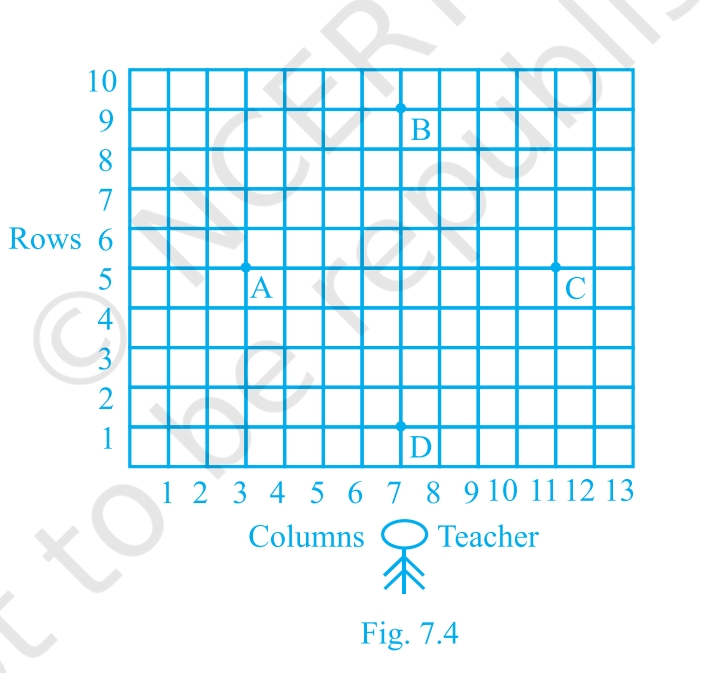
\includegraphics[width=\columnwidth]{figs/sc.jpg}
  \caption{}
\label{fig:10/7/12Fig1}
\end{figure}
\end{enumerate} 
\end{document}
